\documentclass{apnotes}

\title{12 Month Evaluation Report}
\author{Adarsh Pyarelal}
\date{\today}

\begin{document}
\maketitle

\bigskip
\bigskip

\begin{abstract}
  Notes on preparing for the 12 month evaluation.
\end{abstract}

\tableofcontents*

\bigskip
\bigskip


\chapter{CAG Construction Procedure}

The CAG was constructed as follows.

\begin{enumerate}

  \item The preassembled corpus of statements from the four readers (Eidos,
    SOFIA, Hume, and
    CWMS)\footnote{\texttt{wm\_12\_month\_4\_reader\_20190118.json}} was
    deserialized, and filtered through the following selection criteria.

\begin{center}
  \begin{tabular}{lr}
      \toprule
      Stage                                               & Number of statements\\
      \midrule
      Original number of Influence statements             & 18944\\
      Statements with belief score > 0.85                 & 7283\\
      Statements with UN groundings                       & 5808\\
      Statements with subj and obj grounding scores > 0.9 & 184\\
      \bottomrule
  \end{tabular}
\end{center}

\item The \texttt{subj} and \texttt{obj} attributes of the statements that
  survive these filters that do not have polarities recognized by the readers
  are then assigned a default polarity of 1 (positive) to reflect the linguistic
  conventions of the English language, and then assembled into a large CAG.

\item The following nodes:
  \begin{itemize}
    \item \texttt{UN/events/natural/weather/precipitation}
    \item \texttt{UN/events/weather/precipitation}
  \end{itemize}

  \noindent are merged into each other.\footnote{An artifact of an outdated ontology
  mapping for CWMS in INDRA.  This will be fixed in the next version of the
corpus.} In the rest of this report, we will only show the last part of the name
of the terminal node of the ontology (i.e. after the last forward slash) for the
sake of readability, unless there is a need for disambiguation.

\item All edges pointing inwards to the \texttt{precipitation} node are removed.

\item Since in this scenario, we are concerned with the effects of a
  particularly dry lean season, we extract a subgraph of the original CAG
  centered around the \texttt{precipitation} node by conducting a
  breadth-first search to find all directed paths of length 2 that begin at it.

\item We then prune the resulting subgraph using the following algorithm:
  \begin{enumerate}
    \item For each length-2 permutation of nodes in the CAG, construct the list
      of all simple paths between them, with path length up to some cutoff, in
      this case, 2.
    \item For each set of paths between the nodes constructed in the previous
      set, if the set contains more than one member, then remove the length-1
      path in the set if it does not result in either of the nodes being
      disconnected completely from the graph.
  \end{enumerate}

  This procedure is motivated by the observation that the authors of reports 
  for government agencies like the UN often `compress' causal chains in their
  sentences. Thus, if we simply keep all the edges in the CAG, there is bound to
  be some redundancy between causal paths that can potentially hinder a faithful
  mechanistic representation of the system. This step produces the CAG in
  \autoref{fig:precipitation_centered_cag}.

\item We then map the concepts to indicators using a tool based on word
  embeddings. All the mappings are automated, except for the following:
  
  \bigskip

  {\centering
  \begin{tabular}{lll}
    \toprule
    Concept                     & Indicator                            & Source\\
    \midrule
    \texttt{precipitation}      & Average Total Daily Rainfall (Maize) & DSSAT\\
    \texttt{food\_security}     & IPC Phase Classification             & FEWSNET\\
    \texttt{food\_availability} & Production Meat indigenous, total    & FAO\\
    \texttt{food\_production}   & Production (Maize)                   & DSSAT\\
    \texttt{market}             & Inflation Rate                       & ieconomics.com\\
    \texttt{death}              & Battle-related deaths                & WDI\\
    \bottomrule
  \end{tabular}
  }

\item After this mapping, we proceed to parameterize the indicators, for April
  2017, South Sudan. The parameterization algorithm is designed to not result in
  null values, by allowing for fallback aggregation axes.
\end{enumerate}

\begin{figure}
  \centering
  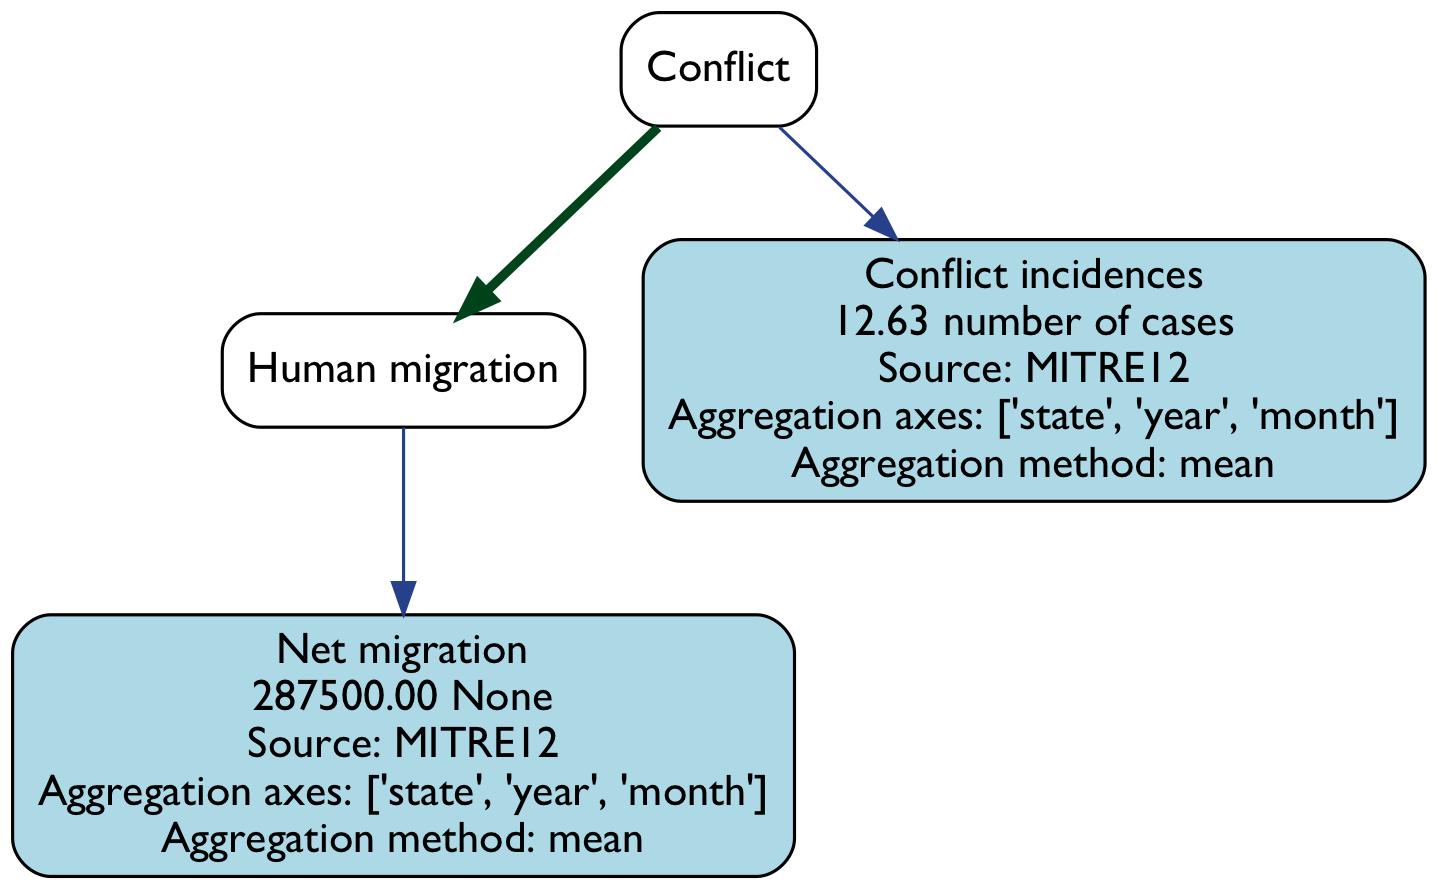
\includegraphics[width=6.5in]{CAG.pdf}
  \caption{Concept-level CAG}
  \label{fig:precipitation_centered_cag}
\end{figure}

\begin{figure}
  \centering
  \includegraphics[width=6.5in]{CAG_with_indicators.pdf}
  \caption{CAG with indicators}
\end{figure}

\begin{figure}
  \centering
  \includegraphics[width=6.5in]{CAG_with_indicators_and_values.pdf}
  \caption{CAG with indicators and values}
\end{figure}

\begin{figure}
  \includegraphics[width=0.4\textwidth]{UN_interventions_humanitarian_assistance.pdf}
\includegraphics[width=0.4\textwidth]{UN_entities_food_availability.pdf}
\includegraphics[width=0.4\textwidth]{UN_entities_human_financial_economic_market.pdf}
\includegraphics[width=0.4\textwidth]{UN_interventions_institutional_support.pdf}
\includegraphics[width=0.4\textwidth]{UN_entities_human_financial_economic_poverty.pdf}
\includegraphics[width=0.4\textwidth]{UN_interventions_provision_of_goods_and_services.pdf}
\includegraphics[width=0.4\textwidth]{UN_entities_human_infrastructure_transportation_road.pdf}
\includegraphics[width=0.4\textwidth]{UN_events_human_agriculture_food_production.pdf}
\includegraphics[width=0.4\textwidth]{UN_entities_human_food_food_security.pdf}
\includegraphics[width=0.4\textwidth]{UN_events_human_death.pdf}

  \caption{Relative changes in the values of the real-valued variables
  representing the abstract concepts in the node, after two time steps. All the
  variables started out at 1.0, with their partial derivatives with respect to
  time set to 0.0, with the exception of the precipitation node, which was set
  to 0.1.}
\end{figure}
\end{document}
